\documentclass[tikz, border=3.14mm]{standalone}
\usepackage{pgfplots}
\pgfplotsset{compat=1.18}

\begin{document}
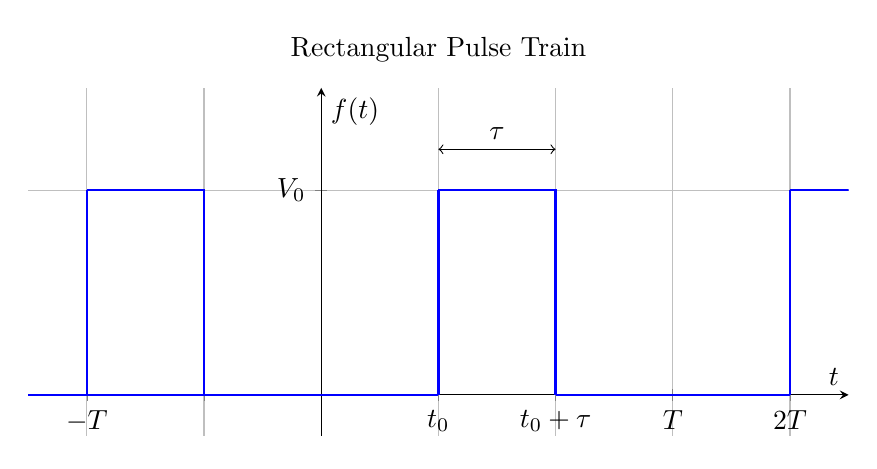
\begin{tikzpicture}
    \begin{axis}[
        axis lines = middle,
        xlabel = {$t$},
        ylabel = {$f(t)$},
        xmin = -2.5, xmax = 4.5,
        ymin = -0.2, ymax = 1.5,
        xtick = {-2, -1, 0, 1, 2, 3, 4},
        xticklabels = {$-T$, , $0$, $t_0$, $t_0+\tau$, $T$, $2T$},
        ytick = {1},
        yticklabels = {$V_0$},
        grid = major,
        width = 12cm,
        height = 6cm,
        title = {Rectangular Pulse Train}
    ]
        % Pulse train: period T, duration tau, amplitude V0
        % Let's assume T=3, tau=1, t0=1 for visualization
        
        % Pulses
        \foreach \n in {-1, 0, 1} {
            \addplot[thick, blue, const plot] coordinates {
                (\n*3 + 1, 1)
                (\n*3 + 2, 1)
                (\n*3 + 2, 0)
            };
            \addplot[thick, blue] coordinates {
                (\n*3 + 1, 0)
                (\n*3 + 1, 1)
            };
        }
        
        % Horizontal lines at zero
        \addplot[thick, blue] coordinates {(-2.5, 0) (1, 0)};
        \addplot[thick, blue] coordinates {(2, 0) (4, 0)};
        \addplot[thick, blue] coordinates {(5, 0) (4.5, 0)};
        
        % Label tau
        \draw[<->] (axis cs:1, 1.2) -- node[above] {$\tau$} (axis cs:2, 1.2);

    \end{axis}
\end{tikzpicture}
\end{document}
